% !TEX root = Bachelorarbeit_Paul_Zilewitsch.tex
\begin{flushright}
Anhang 1\\
Blatt 1\\
\end{flushright}

\noindent Einige Exchange Verbindungen
\begin{flushleft}
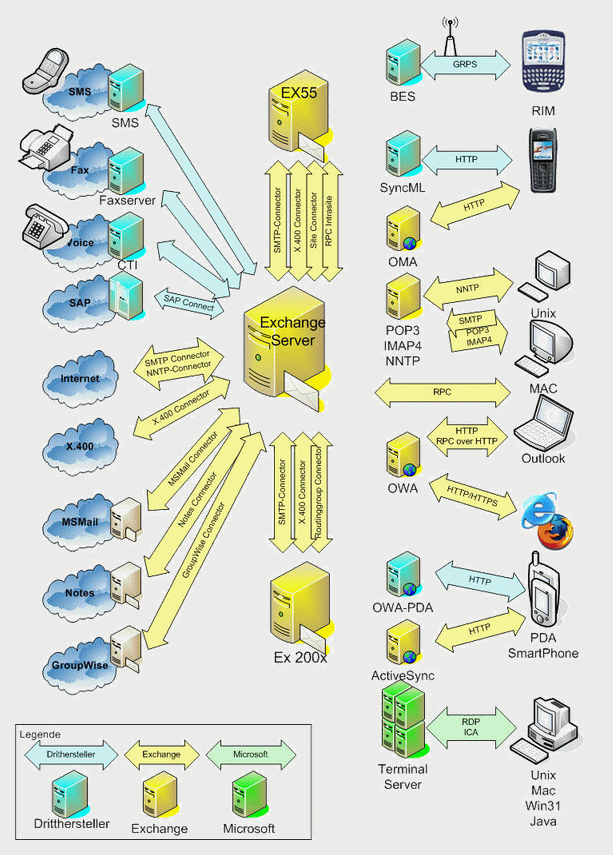
\includegraphics[width=0.65\textwidth]{Abbildungen/Exchange_Verbindungen.png}
\end{flushleft}
\label{Exchange Verbindung}
\noindent Quelle: http://www.msxfaq.de/basics/excomm.htm

\newpage

\begin{flushright}
Anhang 2\\
Blatt 2\\
\end{flushright}

\noindent Übersicht verschiedener APIs
\begin{flushleft}
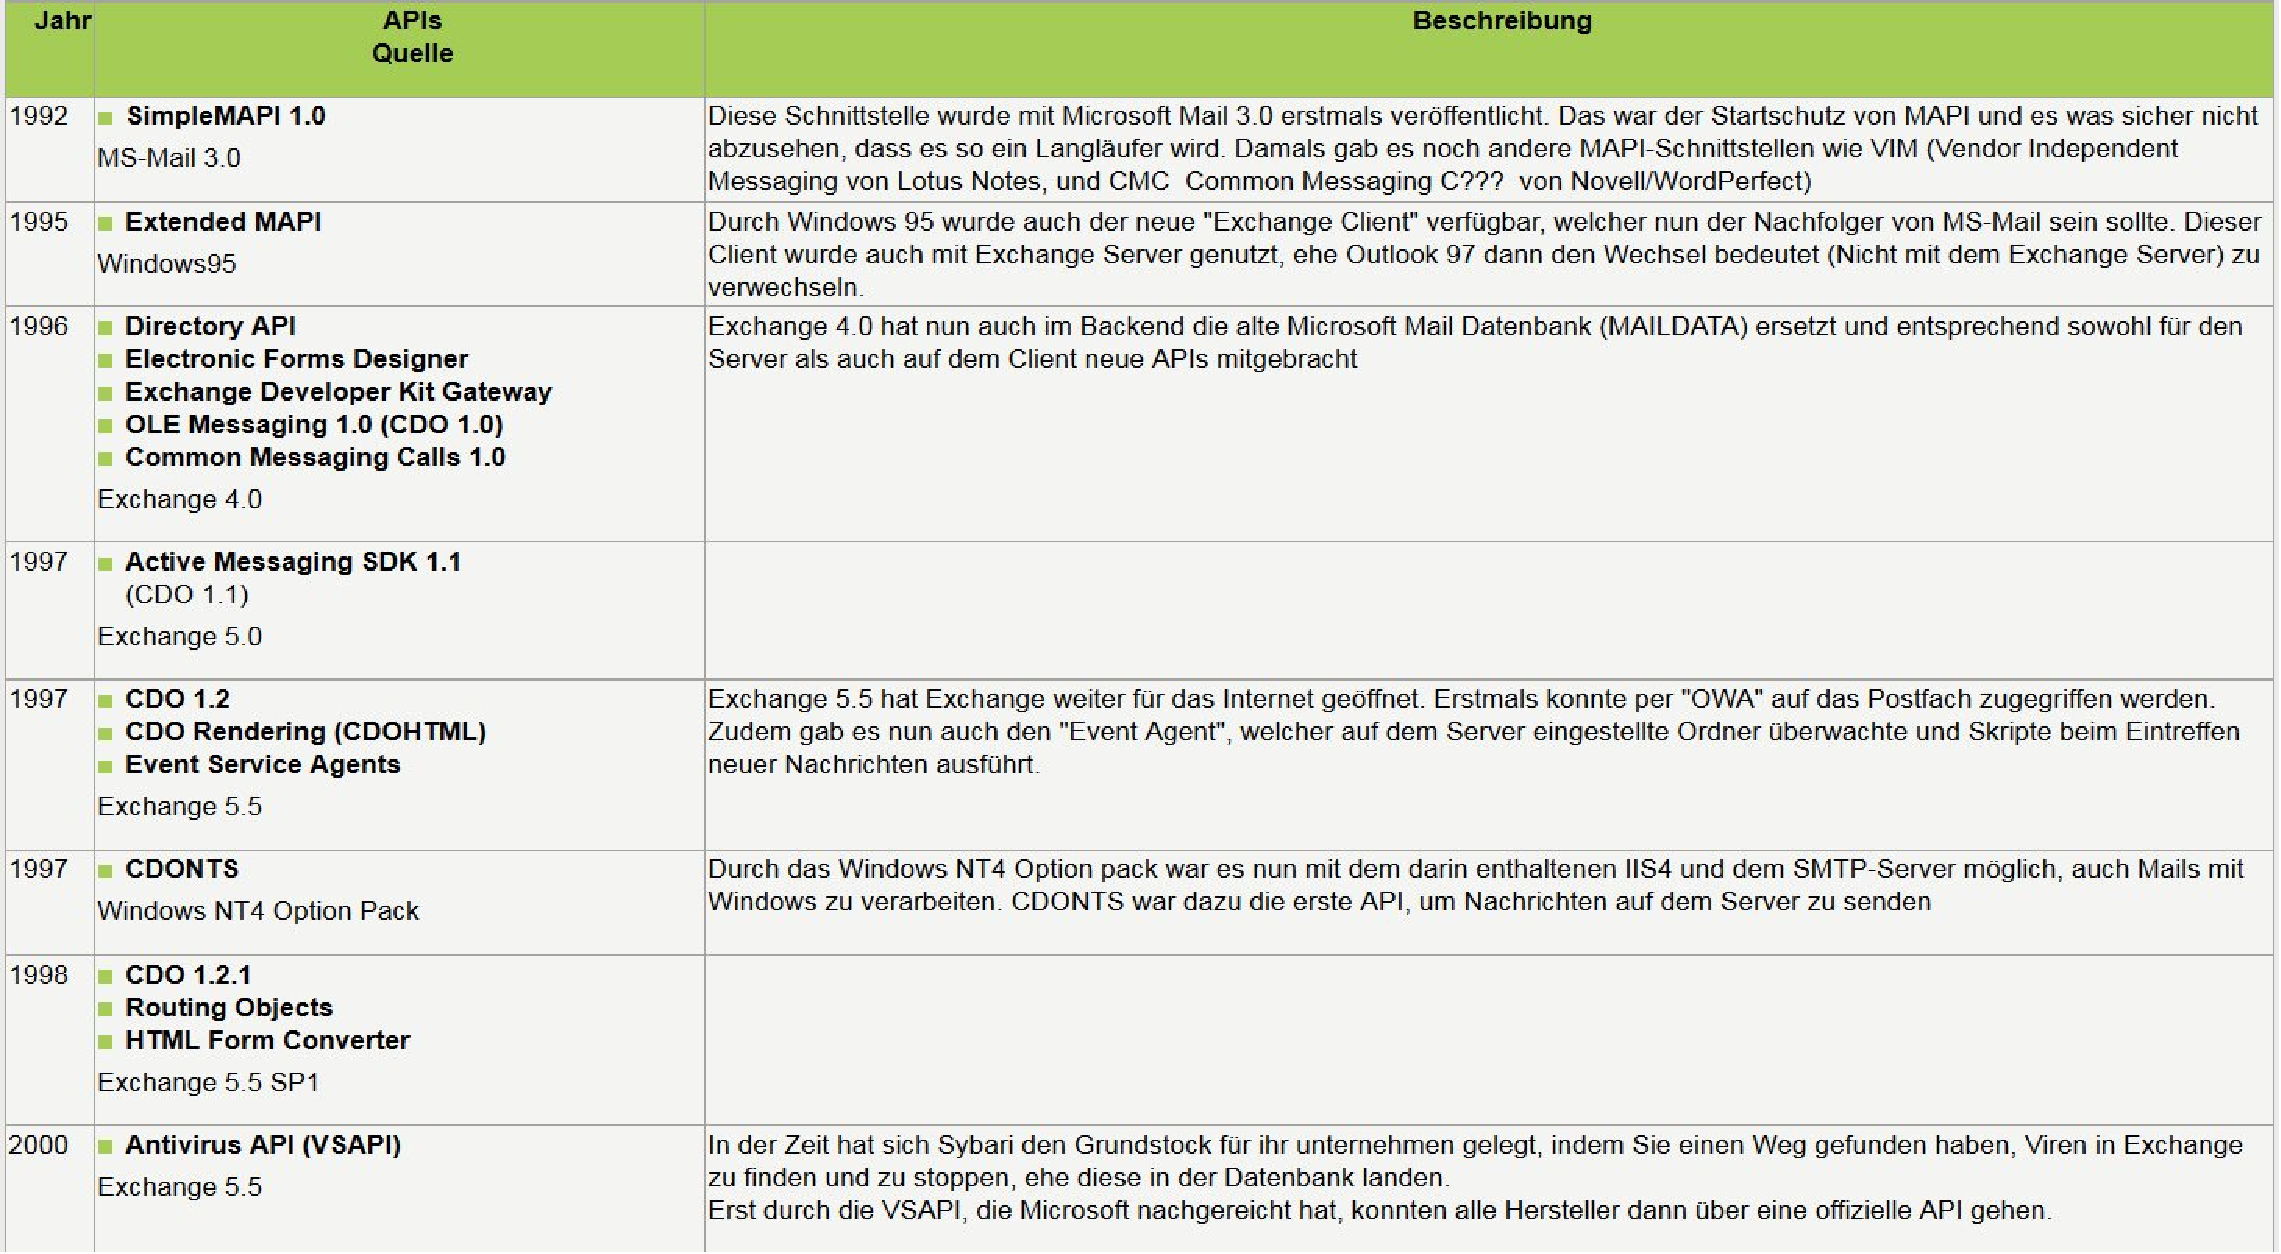
\includegraphics[width=1.0\textwidth]{Abbildungen/API_1.png}
\end{flushleft}
\label{API_1}
\begin{flushleft}
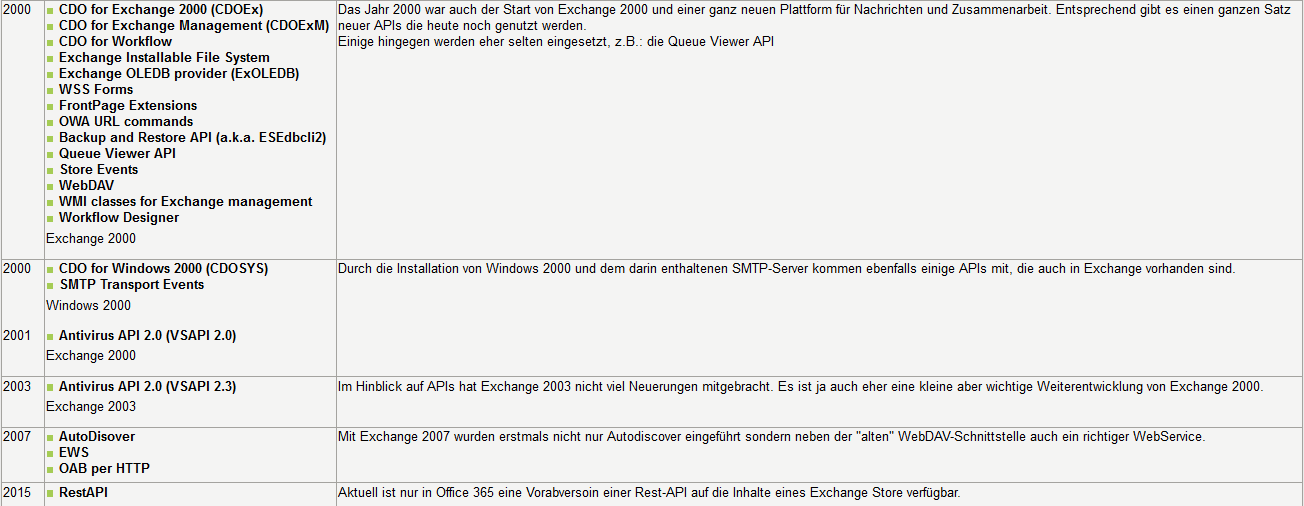
\includegraphics[width=1.0\textwidth]{Abbildungen/API_2.png}
\end{flushleft}
\noindent Quelle: http://www.msxfaq.de/code/wege.htm

\newpage

\begin{flushright}
Anhang 3\\
Blatt 3\\
\end{flushright}

\newpage

\begin{flushright}
Anhang 4\\
Blatt 6\\
\end{flushright}

\newpage

%-------------------------------------------------------------------------------------------------------
%					Literaturverzeichnis
%-------------------------------------------------------------------------------------------------------
\addsec{Literaturverzeichnis} %vergebe keine Kapitelnummer
\noindent
Widl, M (2015): Mircosoft Office 365. Das umfassende Handbuch, 3., aktualisierte Auflage, Bonn\\
\noindent
Joos, T. (2013): Microsoft Exchange Server 2013 - Das Handbuch, Köln

% Recherche Websiten für Service Desk
\noindent
http://venturebeat.com/2014/01/22/help-desk-software-heres-some-of-the-best-and-most-interesting/, 22. Mai 2014

\noindent
http://web.appstorm.net/roundups/communication-roundups/10-online-support-and-help-desk-apps/, 20. März 2015

\noindent
http://www.capterra.com/help-desk-software/ , Oktober 2015

\noindent
http://www.pcmag.com/article2/0,2817,2489457,00.asp , 22. März 2016
